\chapter{Vergleich der verschiedenen Implementierungen}
\label{chapter:4}

In diesem Kapitel wollen wir zum einen konkret auf die Unterschiede eingehen und zum anderen die Laufzeit abhängig von der Anzahl der zu verarbeitenden Datensätze evaluieren.

\section{Benchmarking}
\label{section:4:1}

Nun wollen wir die konkreten Laufzeiten für die implementierten Algorithmen vergleichen. Zu erwarten ist auf jeden Fall, dass Skripte unter Verwendung von iterativen Verfahren länger laufen als solche mit expliziter Berechnung.

Zur Berechnung der Laufzeiten erfolgt erneut mit einem Python-Skript. Dieses Skript führt die jeweilige Regression über einen Kommandozeilenbefehl aus und misst die Zeit dieser Operation. Die Anzahl der Wiederholungen und die Anzahl der verwendeten Datenpunkte können als Parameter übergeben werden. Die Ergebnisse der Berechnungen werden als csv-Datei gespeichert. Das Skript findet man im Anhang unter \ref{appendix:F:1}.

Auch für das Auswerten der berechneten Benchmarks wurde ein Python-Skript erstellt. Dieses Skript liest eine csv-Datei mit Benchmarks und gibt eine Tabelle mit den Werten für jede Art der Regression aus. Außerdem werden mehrere Plots für die Laufzeiten erzeugt. Alle Benchmarks wurden auf einem MacBook Pro (Mitte 2012, Betriebssystem macOS High Sierra 10.13.2) mit einem 2,9 GHz Intel Core i7 Prozessor und 8 GB 1600 MHz DDR3 Arbeitsspeicher berechnet.

\subsection{Einfache lineare Regression}
\label{subsection:4:1:1}

Folgende Ergebnisse erhalten wir bei einfacher linearer Regression:

\begin{center}
  \captionof{table}{Laufzeiten für einfache lineare Regression}
  \begin{tabular}{|c|c|c|c|c|c|}\hline
    & \textbf{10} & \textbf{100} & \textbf{1000} & \textbf{10000} & \textbf{100000} \\ \hline
    \textbf{r} & 0.38453477 & 0.40336191 & 0.38638819 & 0.40475887 & 0.54730985 \\ \hline
    \textbf{tensorflow} & 2.96190362 & 2.94665535 & 3.00290149 & 3.69807061 & 7.73616447 \\ \hline
    \textbf{mysql} & 0.02591379 & 0.02506811 & 0.03348756 & 0.11362195 & 0.82149320 \\ \hline
    \textbf{postgresql} & 0.03092405 & 0.03056195 & 0.03340294 & 0.04948901 & 0.21394655 \\ \hline
  \end{tabular}
\end{center}

Der zugehörige Graph sieht folgendermaßen aus:

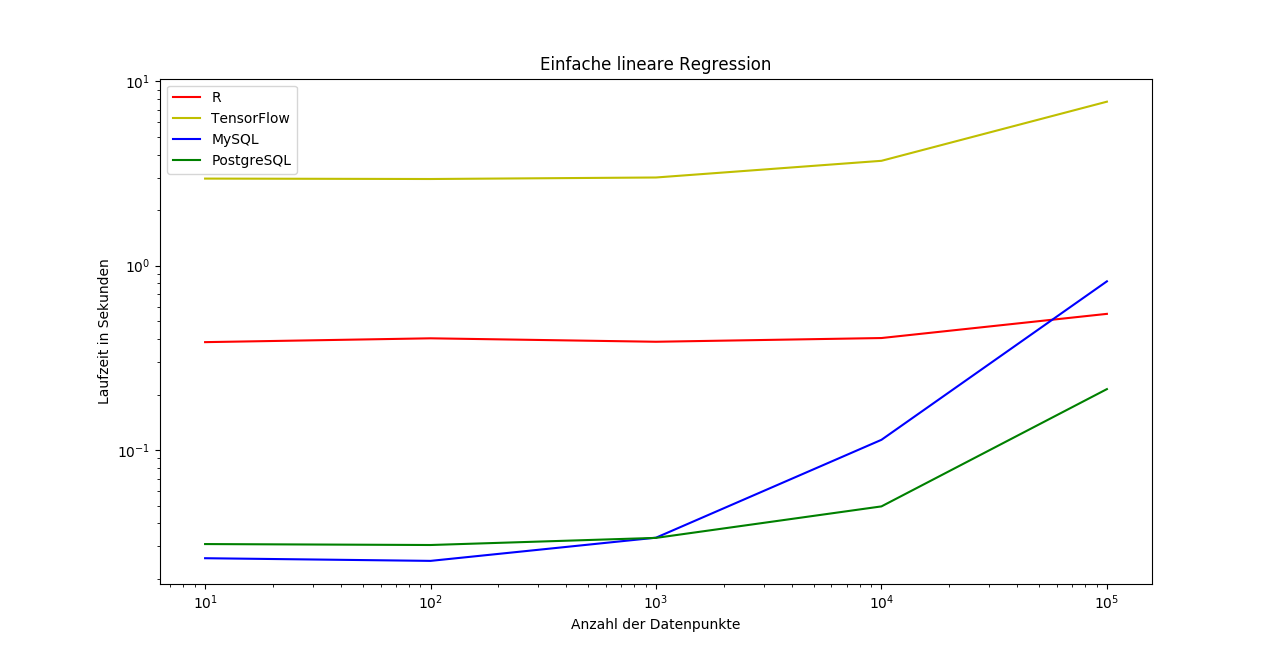
\includegraphics[width=\textwidth]{simpleLinearRegressionBenchmark}

TensorFlow und R haben eine relativ konstante Lautzeit, auch bei größeren Datenmengen. Dabei ist TensorFlow mit iterativer Berechnung wie erwartet mit Abstand am langsamsten. Die SQL-Implementierungen sind bei geringer Anzahl an Datenpunkten sogar die schnellsten Skripte. Für größer werdende Datenmengen erkennt man aber einen rapiden Anstieg in der Laufzeit.

\subsection{Multiple lineare Regression}
\label{subsection:4:1:2}

Die Skripte für multiple lineare Regression besitzen folgende Laufzeiten:

\begin{center}
  \captionof{table}{Laufzeiten für multiple lineare Regression}
  \begin{tabular}{|c|c|c|c|c|c|}\hline
    & \textbf{10} & \textbf{100} & \textbf{1000} & \textbf{10000} & \textbf{100000} \\ \hline
    \textbf{r} & 0.38108478 & 0.37967851 & 0.38452695 & 0.39888490 & 0.54517789 \\ \hline
    \textbf{tensorflow} & 167.220486 & 168.885465 & 168.668689 & 168.821214 & 169.254182 \\ \hline
    \textbf{mysql} & 0.04174929 & 0.05248516 & 0.15990342 & 1.09634777 & 10.8214030 \\ \hline
    \textbf{postgresql} & 0.03053954 & 0.03336087 & 0.05904620 & 0.30572490 & 2.71992954 \\ \hline
  \end{tabular}
\end{center}

Das geplottete Ergebnis sieht wie folgt aus:

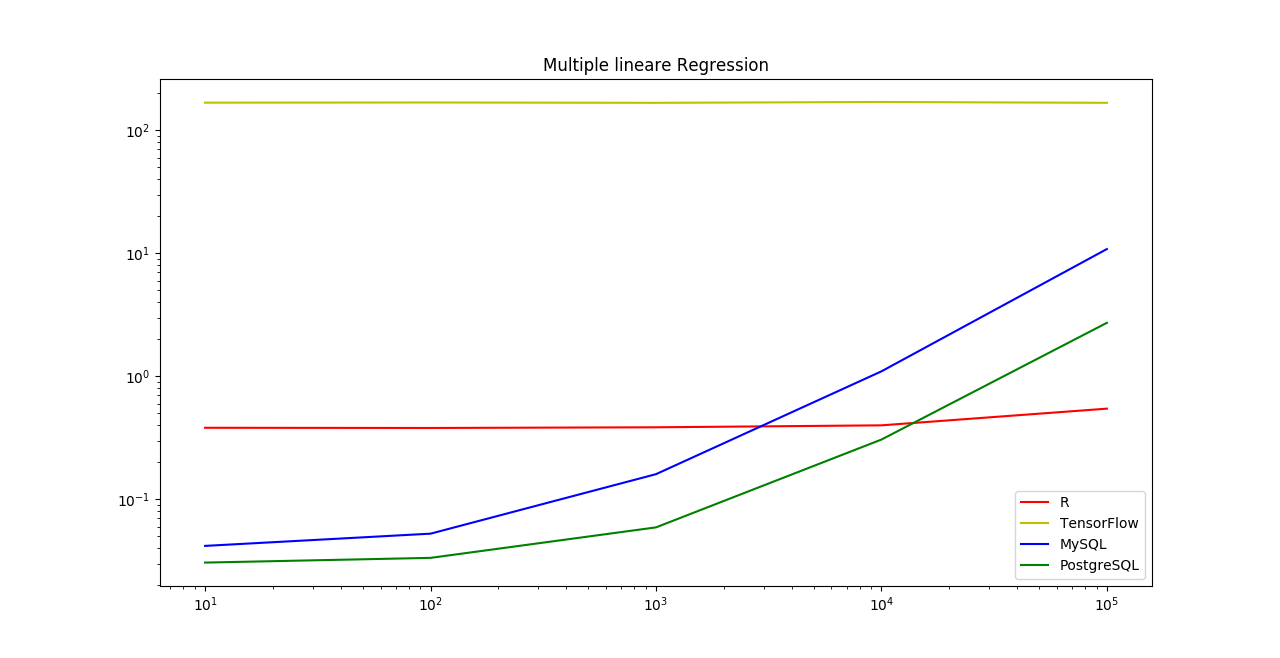
\includegraphics[width=\textwidth]{multipleLinearRegressionBenchmark}

Hier zeigt sich ein ähnliches Bild wie schon bei einfacher linearer Regression. Wieder liefern R und TensorFlow relativ konstante Laufzeiten, wobei die Laufzeit des TensorFlow-Skriptes wegen den $50.000$ durchgeführten Iterationen dieses Mal extrem langsam ist. Wieder sind die SQL-Skripte bei kleinen Datenmengen am schnellsten. Bei größeren Datenmengen werden sie allerdings von R geschlagen. Interessant ist außerdem, dass die PostgreSQL-Implementierung noch schneller als die Variante in MySQL. Die Arrays von PostgreSQL arbeiten also effizienter als die temporären Relationen in MySQL.

\subsection{Logistische Regression}
\label{subsection:4:1:3}

Betrachten wir zuletzt noch die Laufzeiten für logistische Regression:

\begin{center}
  \captionof{table}{Benchmarks für logistische Regression}
  \begin{tabular}{|c|c|c|c|c|c|}\hline
    & \textbf{10} & \textbf{100} & \textbf{1000} & \textbf{10000} & \textbf{100000} \\ \hline
    \textbf{r} & 0.40403676 & 0.39953323 & 0.40047518 & 0.43356463 & 0.91014730 \\ \hline
    \textbf{tensorflow} & 2.88191271 & 2.88278436 & 2.92470042 & 3.37794654 & 6.87024382 \\ \hline
    \textbf{mysql} & 1.57908838 & 4.51631200 & 35.3472805 & 283.849979 & 2680.43056 \\ \hline
    \textbf{postgresql} & 3.73521209 & 48.8452754 & 521.625671 & 5175.87997 &  \\ \hline
  \end{tabular}
\end{center}

Die Visualisierung der Tabelle sieht so aus:

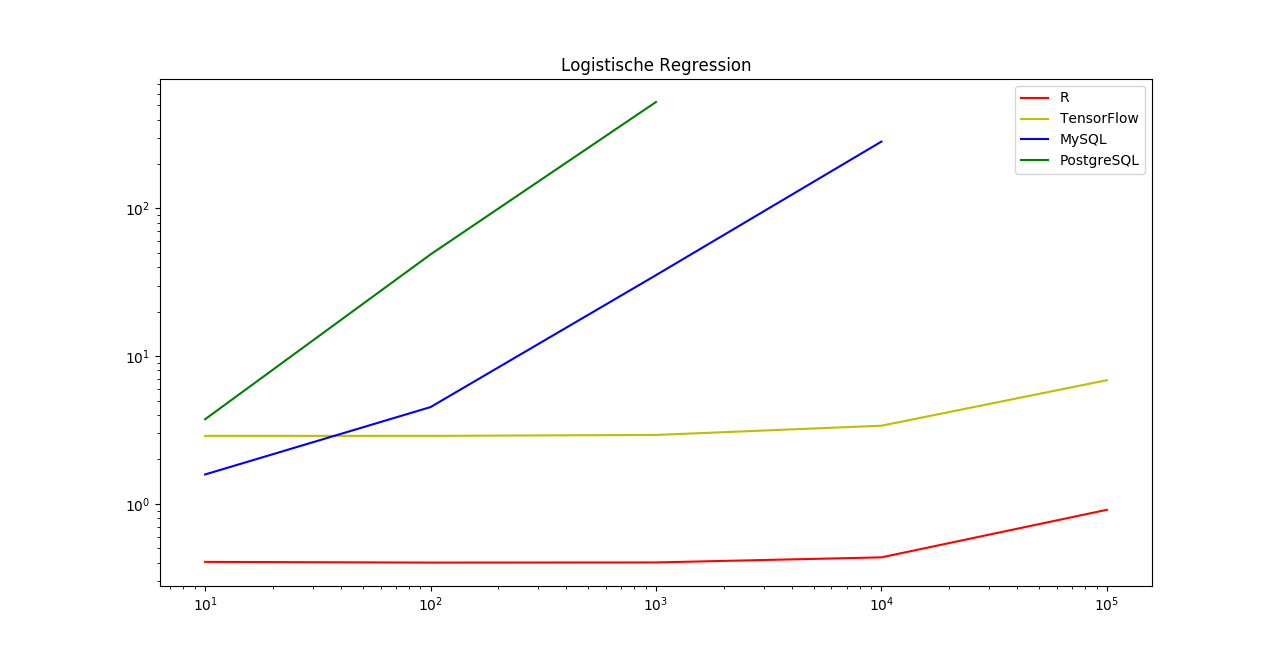
\includegraphics[width=\textwidth]{logisticRegressionBenchmark}

Wieder erkennt man eine Ähnlichkeit zu den vorherigen Diagrammen. Die SQL-Implementierungen sind nun aber von Anfang an deutlich langsamer als die Skripte in R und TensorFlow. Die Laufzeit steigt außerdem sehr schnell weiter an. So wurden für $100.000$ Datenpunkte in PostgreSQL gar keine Benchmarks mehr berechnet, da die erwartete Laufzeit etwa $50.000$ Sekunden, also knapp 14 Stunden beträgt. Klarer Gewinner ist hier R, wo auch $100.000$ Datenpunkte in weniger als einer Sekunde verarbeitet werden können.
